
\chapter{绪论}
\label{chap:introduction}
\section{研究背景与意义}
	自互联网诞生以来,用户寻找信息的方法经历了几个阶段。早期的用户主要靠直接记住感兴趣网站的网址来寻找内容,直接促使Yahoo!提出了分类目录系统,将网站分门别类方便用户查询。但随着信息越来越多,分类目录也只能记录少量的网站,于是产生了搜索引擎。以Google为代表的搜索引擎可以让用户通过关键词找到自己需要的信息,但是,搜索引擎需要用户主动的提供显式关键词来寻找信息,因此它不能解决用户的更多的潜在需求,当用户无法精准描述自己的需求时,搜索引擎就无能为力了,于是又催生出推荐系统\citep{recmd-system}。以亚马逊电商官网为代表的推荐系统是一种帮助用户快速发现有用信息的工具,和搜索引擎不同的是推荐系统不需要提供明确的需求,而是通过分析用户的历史行为来给用户画像建模\citep{demo-data}从而主动给用户推荐出能够满足他们兴趣和需求的信息。因此,从某种意义上说推荐系统和搜索引擎是两个互补的工具。搜索引擎满足用户显式的需求,而推荐系统能够在用户没有明确目的的时候帮助他们发现潜在的需要。随着物联网和用户终端设备的发展,人们逐渐从信息的匮乏时代走进了信息的过载时代。无论是作为信息消费者的普通用户,还是作为信息生产者的提供商面临着数据爆炸时代的挑战。作为用户,如何从充斥着大量噪声的大数据中找到自己感兴趣的信息是一件非常耗时费力的事情,笔者曾有过这样的一种购物体验:在淘宝商城购买一台笔记本电脑,花费了一上午的时间才浏览、比较完所有的 thinkpad 品牌商家店面,如\autoref{fig:hl_taobao}。
	\begin{figure}
		\centering
		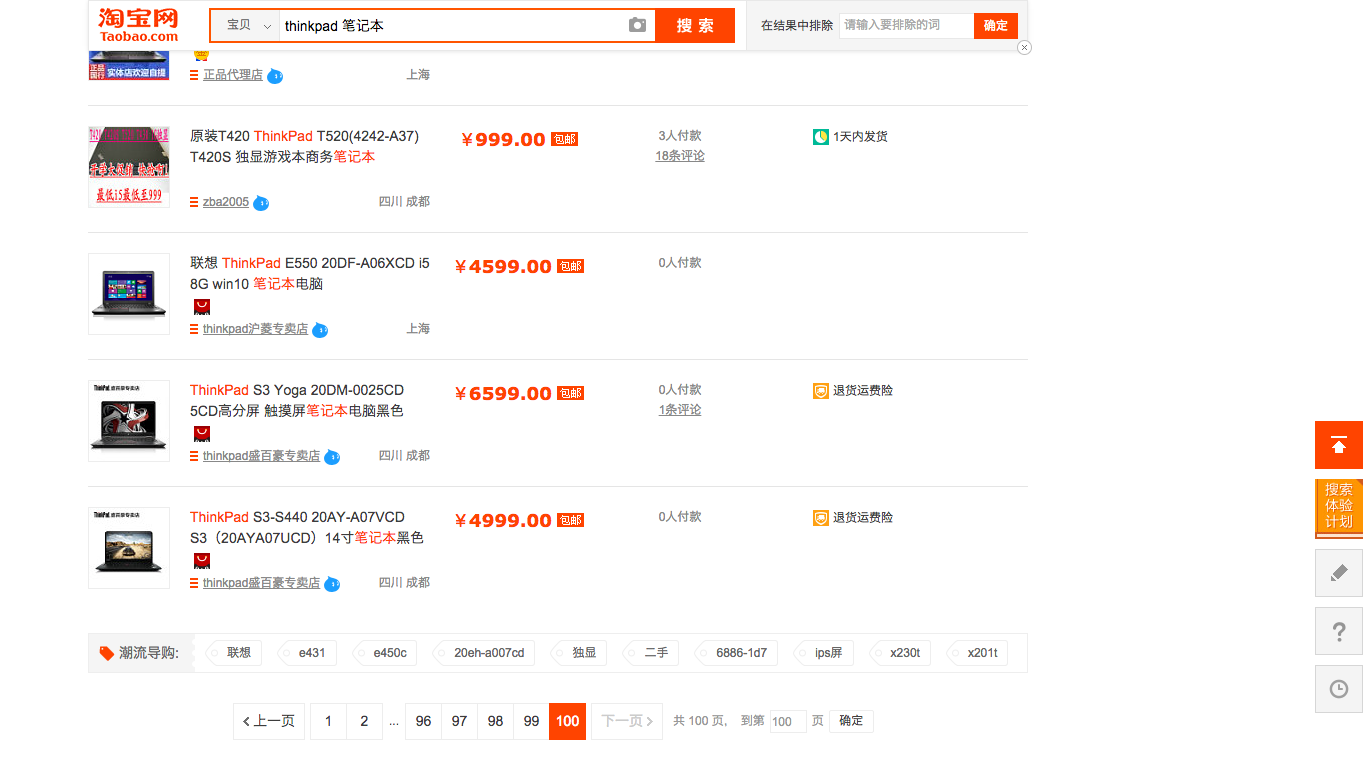
\includegraphics[width=0.9\textwidth]{hl_taobao}
		\figcaption{淘宝购物搜索图}
		\label{fig:hl_taobao}
	\end{figure}

	而近年来淘宝的交易额增长规模巨大,2005年淘宝交易额为80亿,2010年为4000亿,而到2015年淘宝双十一单日交易额就为912亿元,可见未来几年内笔者的这种关键字搜索+逐条浏览的购物方式已经不再具有可行性。而作为提供商,如何让自己生产的信息不埋没在大数据洪流中而受到潜在用户的充分关注,这也是其所要解决的一个课题,很多企业已经或者正在开发适合本公司的推荐系统(Recommender System)来解决这一矛盾。

	推荐系统广泛应用于电子商务领域,通过分析用户的数据,帮助用户找到喜欢和感兴趣的商品,然后推荐给他们。推荐系统的最大优点在于它能收集用户的兴趣信息并根据用户的不同偏好,主动的为用户做出个性化推荐,而且此推荐信息是动态更新的,也就是说随着时间的推移,用户的兴趣在逐渐改变,推荐系统的推荐结果也会随之改变。因此,推荐系统大大的提高了网站的用户体验,方便了用户对资源信息的查询。推荐系统的主要任务就是联系用户和信息,一方面协助用户发现自己潜在感兴趣的信息从而提升用户的满意度,另一方面让信息针对性的展现在只对它有兴趣的用户面前从而提升商品的转化率,于是实现了消费者和生产者的双赢。

	\subsection{推荐系统的定义}
	推荐系统的研究和很多早期的研究相关,比如认知科学(cognitive science)\citep{cognitive-science},信息检索(information retrieval)和预测理论\citep{Forecast-principle}。随着互联网的兴起,研究人员开始研究如何利用用户对物品行为数据来预测用户的兴趣并给用户做推荐\citep{cf-sn}。推荐系统开始成为一个比较独立的研究问题。到2006年为止推荐系统的研究主要集中在基于邻域的协同过滤算法,目前工业界应用最广泛、最知名的算法应该就是亚马逊开发并使用的协同过滤算法\citep{Amazon-cf}。推荐系统推荐给用户的商品首先不能与用户购买过的商品重复,其次也不能与用户刚浏览过的商品太相关。推荐系统的形式化定义如:设C是所有用户的集合,S是所有可以推荐给用户的主题的集合。实际上,C和S集合的规模通常很大,如上百万的顾客以及上万款手机主题。设函数u()可以计算主题s对用户c的推荐度R,即$u=C\times S \rightarrow R$,R是一定范围内的全序的非负实数,推荐要研究的问题就是找到推荐度R最大的那些主题S*,如\autoref{equ:fromal}。
	\begin{equation}
	\forall c \in C,S^{*}=arg  max_{s \in S} u(c,s)
	\label{equ:fromal}
	\end{equation}

	\subsection{推荐系统的产生与发展}
	随着科学技术与信息传播的迅猛发展,人类社会进入了一个全新的大数据时代,互联网和物联网无处不在的影响着人类生活的方方面面,并颠覆性改变了人们的生活方式,互联网用户既代表了网络信息的消费者,也代表了网络内容的生产者。尤其是随着Web 2.0时代的到来,社交化网络媒体的异军突起,互联网中的信息量呈指数级增长,而由于用户的辨别能力有限,使得其在庞大且复杂的互联网信息中找寻有用信息的成本巨大,这就是所谓的信息过载问题\citep{info-overload, info-overload:1}。搜索引擎和推荐系统的出现为用户解决信息过载提供了非常重要的技术手段。搜索引擎是被动的,用户在搜索互联网中的信息时需要在搜索引擎中输入关键词,搜索引擎根据输入在系统后台进行信息匹配,将与用户查询相关的信息展示给用户。但是当用户无法精确描述自己需求时,搜索引擎就无能为力了。推荐系统是主动的,用户不需要提供明确的需求,而是通过分析用户的历史行为来对用户进行分析,从而主动给用户推荐可能满足他们兴趣和需求的信息。因此搜索引擎和推荐系统是两个互补的技术手段。

	推荐系统概念是1995年在美国人工智能协会\citep{recmd-history}上由CMU大学的教授Robert Armstrong首先提出并推出了推荐系统的原型系统——Web Watcher。随后推荐系统的研究工作开始慢慢壮大。第一个正式商用的推荐系统是1996年Yahoo网站推出的个性化入口MyYahoo。21新世纪推荐系统的研究与应用随着电子商务的快速发展而风起云涌,各大电子商务网站都开发、部署了推荐系统,Amazon公司称其网站中35\%的营业额来自于自身的推荐系统。2006年美国的DVD租赁公司Netflix\citep{recmd-netflix}在网上公开设立了一个推荐算法竞赛并公开了真实网站中的一部分数据,包含用户对电影的评分。Netflix竞赛有效地推动了学术界和产业界对推荐算法的兴趣,很多有效的算法在此阶段被提了出来。

	自从1992年施乐的科学家为了解决信息负载的问题,第一次提出协同过滤算法,个性化推荐已经经过了二十几年的发展。1998年,林登和他的同事申请了item-to-item协同过滤技术的专利,经过多年的实践,亚马逊宣称销售的推荐占比可以占到整个销售GMV(Gross Merchandise Volume,即年度成交总额)的30\%以上。随后Netflix举办的推荐算法优化竞赛,吸引了数万个团队参与角逐,期间有上百种的算法进行融合尝试,加快了推荐系统的发展,其中SVD(Sigular Value Decomposition,即奇异值分解,一种正交矩阵分解法)和Gavin Potter跨界的引入心理学的方法进行建模,在诸多算法中脱颖而出。其中,矩阵分解的核心是将一个非常稀疏的用户评分矩阵R分解为两个矩阵:User特性的矩阵P和Item特性的矩阵Q,用P和Q相乘的结果R'来拟合原来的评分矩阵R,使得矩阵R'在R的非零元素那些位置上的值尽量接近R中的元素,通过定义R和R'之间的距离,把矩阵分解转化成梯度下降等求解的局部最优解问题。与此同时,Pandora、LinkedIn、Hulu、Last.fm等一些网站在个性化推荐领域都展开了不同程度的尝试,使得推荐系统在垂直领域有了不少突破性进展,但是在全品类的电商、综合的广告营销上,进展还是缓慢,仍然有很多的工作需要探索。特别是在全品类的电商中,单个模型在母婴品类的效果还比较好,但在其他品类就可能很差,很多时候需要根据品类、推荐栏位、场景等不同,设计不同的模型。同时由于用户、SKU不停地增加,需要定期对数据进行重新分析,对模型进行更新,但是定期对模型进行更新,无法保证推荐的实时性,一段时间后,由于模型训练也要相当时间,可利用传统的批处理的Hadoop的方法是无法再缩短更新频率,最终推荐效果会因为实时性问题达到一个瓶颈。推荐算法主要有基于人口统计学的推荐、基于内容的推荐、基于协同过滤的推荐等,而协同过滤算法又有基于邻域的方法(又称基于记忆的方法)、隐语义模型、基于图的随机游走算法等。基于内容的推荐解决了商品的冷启动问题,但是解决不了用户的冷启动问题,并且存在过拟合问题(往往在训练集上有比较好的表现,但在实际预测中效果大打折扣),对领域知识要求也比较高,通用性和移植性比较差,换一个产品形态,往往需要重新构建一套,对于多媒体文件信息特征提取难度又比较大,往往只能通过人工标准信息。基于邻域的协同过滤算法,虽然也有冷启动问题和数据稀疏性等问题,但是没有领域知识要求,算法通用性好,增加推荐的新颖性,并且对行为丰富的商品,推荐准确度较高。基于模型的协同过滤算法在一定程度上解决了基于邻域的推荐算法面临的一些问题,在RMSE(Root Mean Squared Error,即均方根误差)等推荐评价指标上更优,但是通常算法复杂,计算开销大,所以目前基于邻域的协同过滤算法仍然是最为流行的推荐算法。

	自推荐系统诞生后学术界对其关注的兴趣度也越来越大。从1999年开始美国计算机学会每年召开电子商务研讨会以来,发表的与推荐系统相关的论文数以千计。ACM信息检索专业组在2001年开始把推荐系统作为该会议的一个独立研究主题。同年召开的人工智能联合大会也将推荐系统作为一个单独的主题。目前为止数据库、数据挖掘、人工智能、机器学习方面的重要国际会议(如KDD、AAAI、ICML等)都有大量与推荐系统相关的研究成果发表。同时第一个以推荐系统命名的国际会议ACM Recommender Systems Conference 于2007年首次举办。在近几年的数据挖掘及知识发现国际会议举办的竞赛中,连续两年的竞赛主题都是推荐系统。2011年的KDD CUP 竞赛中,两个竞赛题目分别为音乐评分预测和识别音乐是否被用户评分(\href{http://www.kdd.org/kdd2011/kddcup.shtml}{www.kddcup2011.org})。2012年的KDD CUP 竞赛中,两个竞赛题目分别为腾讯微博中的好友推荐和计算广告中的点击率预测。(\href{www.kddcup2012.org}{www.kddcup2012.org})

	\subsection{推荐系统的作用}
	推荐系统改变了没有活力的网站与其用户通信的方式。无需提供一种静态体验,让用户搜索并可能购买产品,推荐系统加强了交互,以提供内容更丰富的体验。推荐系统根据用户过去的购买和搜索历史,以及其他用户的行为,自主地为各个用户识别推荐内容。个性化推荐的最大的优点在于它能收集用户特征资料并根据用户特征,如兴趣偏好,为用户主动作出个性化的推荐。而且,系统给出的推荐是可以实时更新的,即当系统中的商品库或用户特征库发生改变时,给出的推荐序列会自动改变。这就大大提高了电子商务活动的简便性和有效性,同时也提高了企业的服务水平。总体说来,一个成功的个性化推荐系统的作用主要表现在以下几个方面:
	\begin{enumerate}[(1)]
	\item 将电子商务网站的浏览者转变为购买者:电子商务系统的访问者在浏览过程中经常并没有购买欲望,个性化推荐系统能够向用户推荐他们感兴趣的商品,从而促成购买过程。
	\item 提高电子商务网站的交叉销售能力:个性化推荐系统在用户购买过程中向用户提供其他有价值的商品推荐,用户能够从系统提供的推荐列表中购买自己确实需要但在购买过程中没有想到的商品,从而有效提高电子商务系统的交叉销售。
	\item 提高客户对电子商务网站的忠诚度:与传统的商务模式相比,电子商务系统使得用户拥有越来越多的选择,用户更换商家极其方便,只需要点击一两次鼠标就可以在不同的电子商务系统之间跳转。个性化推荐系统分析用户的购买习惯,根据用户需求向用户提供有价值的商品推荐。如果推荐系统的推荐质量很高,那么用户会对该推荐系统产生依赖。因此,个性化推荐系统不仅能够为用户提供个性化的推荐服务,而且能与用户建立长期稳定的关系,从而有效保留客户,提高客户的忠诚度,防止客户流失。
	\end{enumerate}

	\subsection{推荐系统与电子商务}
	近几年随着电子商务蓬勃发展,推荐系统在互联网中的优势地位也越来越明显。在国外比较著名的电子商务网站有Amazon和eBay,其中Amazon平台中采用的推荐算法是非常成功的。在国内比较典型的电子商务平台网站有淘宝网、网页云音乐、爱奇艺PPS等。在这些电子商务平台中,网站提供的商品数量不计其数,网站中的用户规模也非常巨大。据不完全统计天猫商城中的商品数量已经超过了5000万。在商品数量如此庞大的电商网站中,如果用户仅仅根据自己的购买意图输入关键字查询只会得到很多用户很难区分的相似结果,也不便用户做出选择。因此推荐系统作为能够根据用户兴趣\citep{user-interest}为用户推荐商品的主要途径,从而为用户在购物的选择中提供建议的需求非常明显。目前比较成功的电子商务网站中,都不同程度地利用推荐系统在用户购物的同时为用户推荐一些商品,从而提高商品的销售额。另一方面,随着以智能手机为代表的物联网推动了移动互联网的发展。在用户在连入移动互联网的过程中,其所处的地理位置信息可以非常准确地被获取,并由此出现了大量的基于用户位置信息的网站。国外比较著名的有Uber和Coupons。国内著名的有滴滴出行和美团网。例如,在美团网这种基于位置服务的网站中,用户可以根据自己的当前位置搜索餐馆、酒店、影院、旅游景点等信息服务。同时,可以对当前位置下的各类信息进行点评,为自己在现实世界中的体验打分,分享自己的经验与感受。当用户使用这类基于位置的网站服务时,同样会遭遇信息过载问题。推荐系统可以根据用户的位置信息为用户推荐当前位置下用户感兴趣的内容,为用户提供符合其真正需要的内容,提升用户对网站的满意度。

	随着社交网络的深入人心,用户在互联网中的行为不再局限于获取信息,更多的是与网络上的其他用户进行互动。国外著名的社交网络有Facebook、Twitter等,国内的社交网络有微信、米聊等。在社交网站中用户不再是单个的个体,而是与网络中的很多人具有了错综复杂的社交关系链。社交网络中最重要的资源就是用户与用户之间的这种联系。社交网络中用户间的关系是多维度的,建立社交关系的因素可能是在现实世界中是亲人、同学、同事、朋友关系,也可能只是网络中的虚拟朋友,比如都是有着共同爱好的会员成员。在社交网络中用户与用户之间的联系紧密度反映了用户之间的信任关系,用户不在是一个个体存在,其在社交网络中的行为或多或少地会受到其他用户关系的影响。因此推荐系统在这类社交网站中的研究与应用应该考虑用户社交的影响。

	现如今推荐系统在很多领域得到了广泛的应用,如出租车推荐、商品推荐、美餐推荐、电影推荐和音乐推荐,几乎囊括了人类的吃住行穿四大领域,团购网站美团网早已经利用推荐系统提供面向不同业务的个性化服务:1,猜你喜欢:美团最重要的推荐产品,目标是让用户打开美团App的时候,可以最快找到用户想要的团购服务;2,首页频道推荐:若干频道是固定的,若干频道是根据用户的个人偏好推荐出来的;3,今日推荐个性化推送:美团的个性化推送的产品,目的是在用户打开美团App前,就把用户最感兴趣的服务推送给用户,促使用户点击及下单,从而提高用户的活跃度;4,品类列表的个性化排序:美团首页的那些品类频道区。

\section{大数据时代下的推荐系统}
	虽然推荐系统己经被成功运用在很多大型系统、网站,但是在当前大数据的时代下,推荐系统的面临的场景越来越复杂,推荐系统不仅需要解决传统的数据稀疏、冷启动和动态兴趣问题,还面临由大数据引发的更多、更复杂的实际问题,例如数以亿计的用户数目和海量用户同时访问推荐系统所造成的性能压力,使传统的基于单节点架构的推荐系统不再适用。同时Web服务器处理系统请求在大数据集下变得越来越多,Web服务器响应速度缓慢制约了当前推荐系统为大数据集提供推荐。基于实时模式的推荐在大数据集下也面临着严峻考验,用户难以忍受超过秒级的推荐结果返回时间。传统推荐系统的单一数据库存储技术在大数据集下变得不再适用,急需一种对外提供统一接口、对内采用多种混合模式存储的存储架构来满足大数据集下各种数据文件的存储。并且传统推荐系统在推荐算法上采取的是单机节点的计算方式也不能满足海量用户行为数据的计算需求。大数据本身具有的复杂性、不确定性也给推荐系统带来诸多新的挑战,传统推荐系统的时间效率、空间效率和推荐准确度都遇到严重的瓶颈。

	\subsection{推荐系统的关键技术}
	分布式文件系统。传统的推荐系统技术主要处理小文件存储和少量数据计算,大多是面向服务器的架构,中心服务器需要收集用户的浏览记录、购买记录、评分记录等大量的交互信息来为单个用户定制个性化推荐。当数据规模过大,数据无法全部载入服务器内存时,就算采用外存置换算法和多线程技术,依然会出现I/O上的性能瓶颈,致使任务执行效率过低,产生推荐结果的时间过长。对于面向海量用户和海量数据的推荐系统,基于集中式的中心服务器的推荐系统在时间和空间复杂性上无法满足大数据背景下推荐系统快速变化的需求。大数据推荐系统采用基于集群技术的分布式文件系统管理数据。建立一种高并发、可扩展、能处理海量数据的大数据推荐系统架构是非常关键的,它能为大数据集的处理提供强有力的支持。Hadoop 的分布式文件系统架构是其中的典型。与传统的文件系统不同,数据文件并非存储在本地单一节点上,而是通过网络存储在多台节点上。并且文件的位置索引管理一般都由一台或几台中心节点负责。客户端从集群中读写数据时,首先通过中心节点获取文件的位置,然后与集群中的节点通信,客户端通过网络从节点读取数据到本地或把数据从本地写入节点。在这个过程中由HDFS来管理数据冗余存储、大文件的切分、中间网络通信、数据出错恢复等,客户端根据HDFS 提供的接口进行调用即可,非常方便。
	
	分布式计算框架。集群上实现分布式计算的框架很多,Spark作为推荐算法并行化的依托平台,既是一种分布式的计算框架,也是一种新型的分布式计算编程模型,是一种常见的开源计算框架。其基于内存的MapReduce算法的核心思想是分而治之,把对大规模数据集的操作,分发给一个主节点管理下的各个分节点共同完成,然后通过整合各个节点的中间结果,得到最终结果。计算框架负责处理并行编程中分布式存储、工作调度、负载均衡、容错均衡、容错处理以及网络通信等复杂问题,把处理过程高度抽象为两个函数: map和reduce。map负责把任务分解成多个任务,reduce负责把分解后多任务处理的结果汇总起来。
	
	推荐算法并行化。大型企业所需的推荐算法要处理的数据量非常庞大,从TB级别到PB级甚至更高,腾讯Peacock主题模型分析系统需要进行高达十亿文档、百万词汇、百万主题的主题模型训练,仅一个百万词汇乘以百万主题的矩阵,其数据存储量已达3TB。面对如此庞大的数据,若采用传统串行推荐算法,时间开销太大。当数据量较小时,时间复杂度高的串行算法能有效运作,但数据量极速增加后,这些串行推荐算法的计算性能过低,无法应用于实际的推荐系统中。因此,面向大数据集的推荐系统从设计上就应考虑到算法的分布式并行化技术,使得推荐算法能够在海量的、分布式、异构数据环境下得以高效实现。

	\subsection{推荐系统算法简介}
	现有的推荐算法类型很多,但是各有各的局限,因此推荐系统经常采用组合推荐算法,即融合了协同过滤推荐、聚类算法和其他算法的组合推荐算法。
	\begin{enumerate}[(1)]
	\item 协同过滤算法。

	利用用户的历史喜好信息计算用户之间的距离,然后利用目标用户的最近邻居用户对评价的加权评价值来预测目标用户对特定手机主题的喜好程度,系统从而根据这一喜好程度来对目标用户进行推荐。协同过滤是基于这样的假设:为一用户找到他真正感兴趣的内容的好方法是首先找到与此用户有相似兴趣的其他用户,然后将他们感兴趣的内容推荐给此用户。协同过滤正是把这一思想运用到手机推荐系统中来,基于其他用户对某一类手机主题的评价来向目标用户进行推荐。基于协同过滤的推荐系统可以说是从用户的角度来进行相应推荐的,而且是自动的,即用户获得的推荐是系统从购买模式或浏览行为等隐式获得的,不需要用户努力地找到适合自己兴趣的推荐信息,如填写一些调查表格等。

	协同过滤的根本原理是,人们可以从和自己有相同品味、习性的人群那里获得高质量的推荐。协同过滤算法主要研究如何聚类具有相似兴趣特征的人群并基于此做出推荐,因为算法本身是基于用户社交群体,因此往往会涉及到大规模的用户行为数据的计算。协同过滤的应用领域也很广:电子商务,金融信贷,搜素引擎,互联网企业,网络社区等需要对用户提供个性化体验的服务商。因为中国现有的人口国情,协同过滤算法往往需要面对亿万级用户和海量的用户-主题交互数据。作为输入数据,一个用户是以一个N维度的向量来表示,N代表所有的主题数量。向量内容可以为正也可为负,分别表示了用户喜欢、讨厌该主题的程度。对于热门主题,给其打分的用户会很多,其分数应该乘以一个因子u得到有效的分数,u代表所有给其打分的用户个数的倒数,大多数用户向量是稀疏的。在协同过滤算法中关键性的一步就是要选择测量的距离,描述集合相似度算法有欧氏距离、闵可夫斯基距离、汉明距离等,其中最常用的有余弦距离公式(cosine similiarity),公式描述如,
	其中$similarity_{uv}$代表用户u与v之间的兴趣相似度,N(u)表示用户u曾经喜欢过的物品集合,N(v)表示用户v曾经喜欢过的物品集合。
	\begin{equation}
	similarity_{uv} = \frac{|N(u)\cdot N(v)|}{||N(u)||\cdot||N(v)||}
	\label{cosine-similiarity}
	\end{equation}
	
	然后利用相似度算法把用户分类成独立的集合,每个用户有且只属于其中的一个集合,对于每个集合,取这个集合最受欢迎的top N 个主题,作为推荐内容推荐给集合的所有用户。大多数情况下协同过滤算法面都临着一个问题:最坏情况下需要遍历所有的用户和所有的主题,算法计算复杂度为O(MN),M是用户数N是主题数,解决方法可以借助一种简单的降维思想加以解决:通过去掉那些非常冷门的主题对N做降维,通过去掉那些非常不活跃的用户对M做降维,计算维度下降的代价是降低了推荐系统的准确性。
	\item 聚类算法

	聚类分析是对于统计数据分析的一门技术,和分类算法一个主要的区别就是聚类不需要人工参与打标签,基于聚类的协同过滤方法,也可以在一定程度上解决传统协同过滤算法用户评分矩阵稀疏和冷启动问题,在降低用户评分矩阵稀疏性的同时提高目标用户最近邻居的查询速度。聚类是把相似的对象通过静态分类的方法分成不同的组别或者更多的子集,这样让在同一个子集中的成员对象都有相似的一些属性,聚类结果不仅可以揭示数据间的内在联系与区别,还可以为进一步的数据分析与知识发现提供重要依据。在结构性聚类中关键性的一步就是要选择测量的距离。一个简单的测量就是使用曼哈顿距离,它相当于每个变量的绝对差值之和。该名字的由来起源于在纽约市区测量街道之间的距离就是由人步行的步数来确定的。聚类模块可以是对用户兴趣属性相似度做聚类,也可以对用户社交属性相似度做聚类,或者俩种兼有。

	在现实社会中人们的兴趣和选择往往受到身边亲朋好友的影响。在互联网中随着诸如国内的腾讯,国外的Twitter等社会网络网站的兴起,如何利用用户的社会属性做推荐是近几年推荐领域比较热门的研究问题。基于社会网络的推荐算法被称为社会化推荐。近几年在工业界已经有了很多社会化推荐系统。最简单的社会化过滤算法是基于邻域的算法。给定用户u,令F(u)为用户u的好友集合,N(u)为用户u喜欢的物品集合。那么用户u对物品i的喜好程度定义为用户u的好友中喜欢物品i的好友个数,如公\autoref{Social-Rec}。
	\begin{equation}
		P_{vi} = \sum_{v\in F(v),i\in N(u)}^{} 1
		\label{Social-Rec}
	\end{equation}

	聚类算法在许多领域受到广泛应用,包括机器学习,数据挖掘,模式识别,图像分析以及生物信息,最常用的k-means算法\citep{recmd-kmeans}表示以空间中k个点为中心进行聚类,对最靠近他们的对象归类。
	\item 基于内容的推荐算法。

	基于内容的推荐是信息过滤技术的延续与发展,它是建立在对手机主题的标签信息上作出推荐的,而不需要依据用户对手机主题的评价意见,需要用机器学习的方法从关于内容的特征描述的事例中得到用户的兴趣资料。手机主题是通过相关的特征的属性来定义,系统基于用户评价对象的特征,学习用户的兴趣,考察用户资料与待预测手机主题的相匹配程度。用户的资料模型取决于所用学习方法,采用了综合决策树、神经网络和基于向量的组合方法。 基于内容的用户资料是需要有用户的历史数据,用户资料模型可能随着用户的偏好改变而发生变化。基于内容推荐方法的优点是:不需要其它用户的数据,没有冷开始问题和稀疏问题。能为具有特殊兴趣爱好的用户进行推荐。能推荐新的或不是很流行的手机主题,没有产品问题。通过列出推荐手机主题的内容特征,可以解释为什么推荐那些手机主题。

	本节利用spark mllib中ALS算法解释基于内容的推荐。首先,给出一个(用户,主题,评分)三元组的数据集,ALS会建立一个user$\ast$product的m$\ast$n的矩阵,其中,m为用户的数量,n为商品的数量。这个矩阵的每一行代表一个用户 ($u_1$,$u_2$,…,$u_9$)、每一列代表一个产品 ($v_1$,$v_2$,…,$v_9$)。用户的打分在0到10之间。但是在这个数据集中,并不是每个用户都对每个产品进行过评分,所以这个矩阵往往是稀疏的,所以需要做预处理将其填满,然后开始训练:
    假设m$\ast$n的评分矩阵R,可以被近似分解成$U*V^{T}$ ,U为m$\ast$d的用户特征向量矩阵,V为n$\ast$d的产品特征向量矩阵,d为用户和商品的特征值的数量。

    \begin{center} 
	$\begin{Bmatrix}
	  & u_1 & u_2\\ 
	p_1 & 8 & 7\\ 
	p_2 & 44 & 39
	\end{Bmatrix} =
	\begin{Bmatrix}
	  & f_1 & f_2\\ 
	p_1 & 0 & 1\\ 
	p_2 & 2 & 3
	\end{Bmatrix} \ast 
	\begin{Bmatrix}
	  & u_1 & u_2\\ 
	p_1 & 10 & 9\\ 
	p_2 & 8 & 7
	\end{Bmatrix}$
	\end{center}

	对于电影类型的手机主题,可以从d个角度进行评价,如主角,铃声,背景,特效4个角度来评价,那么d就等于4。矩阵V由n个product$\ast$d个特征值组成。对于矩阵U,假设对于任意的用户A,该用户对一款手机主题的综合评分和主题的特征值存在一定的线性关系,综合评分=(a1*d1+a2*d2+a3*d3+a4*d4) ,其中$a_{i}$为用户A的特征值,$d_{i}$为之前所说的主题的特征值。ALS算法认为m*n的评分矩阵R可以被近似分解成$U*V^{T}$,得到目标函数:
    \begin{equation}
    L(U,V)=\sum_{i,j}(R_{ij}-U_{i}^{T}V_{j})^{2}
    \label{F-Measure}
    \end{equation}

    其中a表示评分数据集中用户i对产品j的真实评分,另外一部分表示用户i的特征向量和产品j的特征向量,加上正则化参数$\lambda (||U_i||^2+||V_j||^2)$以防止过度拟合,固定V对U求导得到公式:
    \begin{equation}
    U_{t}=R_{t}V_{ut}(V_{ut}^TV_{ut}+\lambda n_{ut}I)^{-1}, i \in [1,m]
    \label{equa-least2}
    \end{equation}

    其中$R_{t}$表示用户i评过的手机主题的评分向量,$V_{ut}$表示用户i评过的手机主题的特征向量组成的特征矩阵。$n_{ut}$表示用户i评过的手机主题数量。同理,固定U,可以得到求解$V_{j}$的公式:
    \begin{equation}
    V_{j}=R_{j}^{T}U_{mj}(U_{mj}^{T}U_{mj}+\lambda n_{mj}I)^{-1}
    \label{equa-least3}
    \end{equation}

    $R_{j}$表示评过手机主题j的用户向量,$U_{mj}$表示评过手机主题j的用户特征向量组成的矩阵,$m_{mj}$表示评过电影j的用户的数量。

    首先用一个小于1的随机数初始化V,根据\autoref{equa-least2}求U,此时就可以得到初始的UV矩阵了,根据计算得到的U和\autoref{equa-least3}重新计算并覆盖V,反复进行以上两步的计算,直到目标函数和小于一个预设的值,或者迭代次数满足要求则停止。
	\item 组合推荐。

	由于各种推荐方法都有优缺点,手机主题推荐采用了组合推荐方式。研究和应用最多的是基于内容的推荐和协同过滤推荐的组合。最简单的做法就是分别用基于内容的方法和协同过滤推荐方法去产生一个推荐预测结果,然后用某方法组合其结果。组合推荐一个最重要原则就是通过组合后要能避免或弥补各自推荐技术的弱点。在组合方式上使用了几种组合思路:加权(Weight):加权多种推荐技术结果。变换(Switch):根据问题背景和实际情况或要求决定变换采用不同的推荐技术。混合(Mixed):同时采用多种推荐技术给出多种推荐结果为用户提供参考。特征组合(Feature combination):组合来自不同推荐数据源的特征被另一种推荐算法所采用。层叠(Cascade):先用一种推荐技术产生一种粗糙的推荐结果,第二种推荐技术在此推荐结果的基础上进一步作出更精确的推荐。特征扩充(Feature augmentation):一种技术产生附加的特征信息嵌入到另一种推荐技术的特征输入中。
	\end{enumerate}

	\subsection{推荐系统面临的问题}
	\begin{enumerate}[(1)]
	\item 特征提取问题。

	推荐系统的推荐对象种类丰富,例如新闻、博客等文本类对象,视频、图片、音乐等多媒体对象以及可以用文本描述的一些实体对象等。如何对这些推荐对象进行特征提取一直是学术界和工业界的热门研究课题。对于文本类对象,可以借助信息检索领域己经成熟的文本特征提取技术来提取特征。对于多媒体对象,由于需要结合多媒体内容分析领域的相关技术来提取特征,而多媒体内容分析技术目前在学术界和工业界还有待完善,因此多媒体对象的特征提取是推荐系统目前面临的一大难题。此外推荐对象特征的区分度对推荐系统的性能有非常重要的影响。目前还缺乏特别有效的提高特征区分度的方法。
	\item 数据稀疏问题。

	现有的大多数推荐算法都是基于用户—物品协同过滤矩阵数据,数据的稀疏性问题主要是指用户—物品评分矩阵的稀疏性,即用户与物品的交互行为太少。一个大型网站可能拥有上亿数量级的用户和物品,用户评分数据总量在面对增长更快的“用户—物品评价矩阵”时,仍然表现出稀疏性,推荐系统研究中的经典数据集MovieLens的稀疏度仅4.5\%, Netflix百万大赛中提供的音乐数据集的稀疏度是1.2\%。这些都是已经处理过的数据集,实际上真实数据集的稀疏度都远远低于1\%。例如, Bibsonomy的稀疏度是0.35\%,Delicious的稀疏度是0.046\%,淘宝网数据的稀疏度甚至仅在0.01\%左右。根据经验,数据集中用户行为数据越多,推荐算法的精准度越高,性能也越好。若数据集非常稀疏,只包含极少量的用户行为数据,推荐算法的准确度会大打折扣,极容易导致推荐算法的过拟合,影响算法的性能。
	\item 冷启动问题。

	冷启动问题是推荐系统所面临的最大问题之一。冷启动问题总的来说可以分为3类:系统冷启动问题、新用户问题和新物品问题。系统冷启动问题指的是由于数据过于稀疏,“用户—物品评分矩阵”的密度太低,导致推荐系统得到的推荐结果准确性极低。新物品问题是由于新的物品缺少用户对该物品的评分,这类物品很难通过推荐系统被推荐给用户,用户难以对这些物品评分,从而形成恶性循环,导致一些新物品始终无法有效推荐。新物品问题对不同的推荐系统影响程度不同:对于用户可以通过多种方式查找物品的网站,新物品问题并没有太大影响,如电影推荐系统等,因为用户可以有多种途径找到电影观看并评分;而对于一些推荐是主要获取物品途径的网站,新物品问题会对推荐系统造成严重影响。通常解决这个问题的途径是激励或者雇佣少量用户对每一个新物品进行评分。新用户问题是目前对现实推荐系统挑战最大的冷启动问题:当一个新的用户使用推荐系统时,他没有对任何项目进行评分,因此系统无法对其进行个性化推荐;即使当新用户开始对少量项目进行评分时,由于评分太少,系统依然无法给出精确的推荐,这甚至会导致用户因为推荐体验不佳而停止使用推荐系统。当前解决新用户问题主要是通过结合基于内容和基于用户特征的方法,掌握用户的统计特征和兴趣特征,在用户只有少量评分甚至没有评分时做出比较准确的推荐。

	\item 马太效应。

	马太效应(Mattnew Effect)是指强者愈强、弱者愈弱的现象,在互联网中引申为热门的产品受到更多的关注,冷门内容则愈发的会被遗忘的现象。很不幸的是推荐系统的出现加剧了互联网商品的马太效应,因为很多商品只有很少的评分,因此很难在推荐系统中应用,导致推荐结果大部分为热门商品。与马太效应相对于的是长尾理论,由美国人克里斯·安德森提出。长尾理论认为,由于成本和效率的因素,当商品储存流通展示的场地和渠道足够宽广,商品生产成本急剧下降以至于个人都可以进行生产,并且商品的销售成本急剧降低时,几乎任何以前看似需求极低的产品,只要有卖,都会有人买。这些需求和销量不高的产品所占据的共同市场份额,可以和主流产品的市场份额相比,甚至更大。
	\end{enumerate}

	\subsection{推荐系统开源项目介绍}
	工欲善其事,必先利器,关于大数据,有很多令人兴奋的事情,但如何分析、利用它也带来了很多困惑。好在开源观念盛行的今天,有一些在大数据领域领先的免费开源技术可供利用。
	\begin{itemize}
		\item Apache Hadoop:Hadoop是一个由Apache基金会所开发的分布式系统基础架构,是一种用于分布式存储和处理商用硬件上大型数据集的开源框架,可让各企业迅速从海量结构化和非结构化数据中获得洞察力。Hadoop的框架最核心的设计就是HDFS和MapReduce。HDFS为海量的数据提供了存储,则MapReduce为海量的数据提供了计算。HDFS有高容错性的特点,并且设计用来部署在低廉的硬件上;而且它提供高吞吐量来访问应用程序的数据,适合那些有着超大数据的应用程序。MapReduce 本身就是用于并行处理大数据集的软件框架,其根源是函数性编程中的 map 和 reduce 函数。它由两个可能包含有许多实例的操作组成。Map 函数接受一组数据并将其转换为一个键/值对列表,输入域中的每个元素对应一个键/值对。
		\item Apache Hive:Hive是建立在 Hadoop 上的数据仓库基础构架。它提供了一系列的工具,可以用来进行数据提取转化加载,这是一种可以存储、查询和分析存储在Hadoop中的大规模数据的机制。Hive定义了简单的类SQL查询语言,称为HQL,它允许熟悉SQL的用户查询数据。同时,这个语言也允许熟悉 MapReduce 开发者的开发自定义的 mapper 和 reducer 来处理内建的 mapper 和 reducer 无法完成的复杂的分析工作,十分适合数据仓库的统计分析。
		\item Apache Spark:Spark是加州大学伯克利分校所开源的类Hadoop的通用并行框架,Spark拥有 Hadoop 所具有的优点;但不同于 Hadoop 的是Job中间输出结果可以保存在内存中,从而不再需要读写HDFS,因此Spark能更好地适用于数据挖掘与机器学习等需要迭代的MapReduce的算法。
		\item Apache Kafka:Kafka 是一种高吞吐量的分布式发布订阅消息系统,它可以处理消费者规模的网站中的所有用户行为流数据。这种用户行为流数据是在现代网络上的许多社会功能的一个关键因素。这些数据通常是由于吞吐量的要求而通过处理日志和日志聚合来解决。对于像Hadoop的一样的日志数据和离线分析系统,但又要求实时处理的限制,Kafka一个可行的解决方案。其目的是通过Hadoop的并行加载机制来统一线上和离线的消息处理,也是为了通过集群机来提供实时的消费。
	\end{itemize}

	\subsection{推荐系统的应用案例}
	近几年随着社会化网络的发展,推荐系统在工业界广泛应用并且取得了显著进步。比较著名的推荐系统应用有:淘宝网的电子商务推荐系统、Youtube的视频推荐系统\citep{recmd-youtube}、网易云音乐推荐系统以及Facebook好友推荐系统。个性化推荐系统具有良好的发展和应用前景。目前,几乎所有的大型电子商务系统,如Amazon、eBay等,都不同程度的使用了各种形式的推荐系统。各种提供个性化服务的Web站点也需要推荐系统的大力支持。在日趋激烈的竞争环境下,个性化推荐系统能有效的保留客户,提高电子商务系统的服务能力。成功的推荐系统会带来巨大的效益。我们每天使用的许多网站中都可找到推荐系统。

	作为全球排名第一的社交网站(\href{https://code.facebook.com/posts/861999383875667/recommending-items-to-more-than-a-billion-people/}{https://code.facebook.com/}),Facebook利用分布式推荐系统来帮助用户找到他们可能感兴趣的页面、组、事件或者游戏等,代表了国外推荐系统的最高发展水平。Facebook中推荐系统所要面对的数据集包含了约1000亿个评分、超过10亿的用户以及数百万的物品,如何在在大数据规模情况下仍然保持良好性能已经成为世界级的难题。Facebook设计了一个全新的推荐系统。Facebook团队之前已经在使用一个分布式迭代和图像处理平台——Apache Giraph。因其能够很好的支持大规模数据,Giraph就成为了Facebook推荐系统的基础平台。在工作原理方面,Facebook推荐系统采用的是流行的协同过滤技术。CF技术的基本思路就是根据相同人群所关注事物的评分来预测某个人对该事物的评分或喜爱程度。从数学角度而言,该问题就是根据用户-物品的评分矩阵中已知的值来预测未知的值。其求解过程通常采用矩阵分解方法。MF方法把用户评分矩阵表达为用户矩阵和物品的乘积,用这些矩阵相乘的结果R’来拟合原来的评分矩阵R,使得二者尽量接近。如果把R和R’之间的距离作为优化目标,那么矩阵分解就变成了求最小值问题。对大规模数据而言,求解过程将会十分耗时。为了降低时间和空间复杂度,一些从随机特征向量开始的迭代式算法被提出。这些迭代式算法渐渐收敛,可以在合理的时间内找到一个最优解。随机梯度下降算法就是其中之一,其已经成功的用于多个问题的求解。SGD基本思路是以随机方式遍历训练集中的数据,并给出每个已知评分的预测评分值。用户和物品特征向量的调整就沿着评分误差越来越小的方向迭代进行,直到误差到达设计要求。因此,SGD方法可以不需要遍历所有的样本即可完成特征向量的求解。交替最小二乘法是另外一个迭代算法。其基本思路为交替固定用户特征向量和物品特征向量的值,不断的寻找局部最优解直到满足求解条件。

	为了利用上述算法解决Facebook推荐系统的问题,原本Giraph中的标准方法就需要进行改变。之前,Giraph的标准方法是把用户和物品都当作为图中的顶点、已知的评分当作边。那么,SGD或ALS的迭代过程就是遍历图中所有的边,发送用户和物品的特征向量并进行局部更新。该方法存在若干重大问题。首先,迭代过程会带来巨大的网络通信负载。由于迭代过程需要遍历所有的边,一次迭代所发送的数据量就为边与特征向量个数的乘积。假设评分数为1000亿、特征向量为100对,每次迭代的通信数据量就为80TB。其次,物品流行程度的不同会导致图中节点度的分布不均匀。该问题可能会导致内存不够或者引起处理瓶颈。假设一个物品有1000亿个评分、特征向量同样为100对,该物品对应的一个点在一次迭代中就需要接收80GB的数据。最后,Giraph中并没有完全按照公式中的要求实现SGD算法。真正实现中,每个点都是利用迭代开始时实际收到的特征向量进行工作,而并非全局最新的特征向量。因此Giraph中最大的问题就在于每次迭代中都需要把更新信息发送到每一个顶点。为了解决这个问题,Facebook发明了一种利用work-to-work信息传递的高效、便捷方法。该方法把原有的图划分为了由若干work构成的一个圆。每个worker都包含了一个物品集合和若干用户。在每一步,相邻的worker沿顺时针方法把包含物品更新的信息发送到下游的worker。这样,每一步都只处理了各个worker内部的评分,而经过与worker个数相同的步骤后,所有的评分也全部都被处理。该方法实现了通信量与评分数无关,可以明显减少图中数据的通信量。而且,标准方法中节点度分布不均匀的问题也因为物品不再用顶点来表示而不复存在。为了进一步提高算法性能,Facebook把SGD和ALS两个算法进行了揉合,提出了旋转混合式求解方法。

	接下来,Facebook在运行实际的A/B测试之间对推荐系统的性能进行了测量。首先,通过输入一直的训练集,推荐系统对算法的参数进行微调来提高预测精度。然后,系统针对测试集给出评分并与已知的结果进行比较。Facebook团队从物品平均评分、前1/10/100物品的评分精度、所有测试物品的平均精度等来评估推荐系统。此外,均方根误差(Root Mean Squared Error, RMSE)也被用来记录单个误差所带来的影响。

	此外,即使是采用了分布式计算方法,Facebook仍然不可能检查每一个用户/物品对的评分。团队需要寻找更快的方法来获得每个用户排名前K的推荐物品,然后再利用推荐系统计算用户对其的评分。其中一种可能的解决方案是采用ball tree数据结构来存储物品向量。all tree结构可以实现搜索过程10-100倍的加速,使得物品推荐工作能够在合理时间内完成。另外一个能够近似解决问题的方法是根据物品特征向量对物品进行分类。这样,寻找推荐评分就划分为寻找最推荐的物品群和在物品群中再提取评分最高的物品两个过程。该方法在一定程度上会降低推荐系统的可信度,却能够加速计算过程。

	最后,Facebook给出了一些实验的结果。在2014年7月,Databricks公布了在Spark上实现ALS的性能结果。Facebook针对Amazon的数据集,基于Spark MLlib进行标准实验,与自己的旋转混合式方法的结果进行了比较。实验结果表明,Facebook的系统比标准系统要快10倍左右。而且,前者可以轻松处理超过1000亿个评分。
\section{研究内容与研究方法}
	推荐系统问题之一是冷启动问题,冷启动问题有三种:用户冷启动、物品冷启动、系统冷启动,本文主要研究用户冷启动问题。经典的算法诸如最近邻的协同过滤算法、PageRank排序算法、关联规则挖掘等算法是给定用户对某些物品的行为数据,给每个用户推荐TOP N个其最喜欢的物品,这种思路对于新注册用户来讲效果不好,因为没有用户行为数据可供分析。解决这个问题的关键是对用户画像建模,实验发现融合用户画像的热门商品推荐是解决冷启动问题的最佳方式。

	推荐系统问题之二是马太效应,即热门商品越来越热,冷门商品越来越冷,在互联网指数级的爆发下信息量极大富余,这更加推动了马太效应的快速形成以及规模的无限扩大,现有的大多数推荐算法更是极大地加速马太效应的形成速度以及规模。我们提出利用用户兴趣探索解决商品的马太效应,提升推荐系统对物品长尾的发掘能力,主要思路是分析用户所有的行为数据,针对冷门商品(冷门商品包含的标签一般是小众标签)的行为会赋予一个倾斜因子,这样会导致兴趣探索标签候选集中的小众标签占大多数,而如果用户对其的满意度也很高,则说明这是一个成功的兴趣探索。这里涉及到的概念包括小众标签的定义和用户满意度的量化,将会在用户兴趣探索章节详细介绍。

	推荐系统问题之三是用户兴趣的动态变化问题,即时效性问题。笔者一直关心的一个问题就是不同系统的用户行为究竟有什么区别,并如何根据这些区别来选择合适的时间参数来预测用户的行为。如nytimes的时效性很短,大部分新闻都是在第一天被很多人关注,而后面就没有人关注了,所以即使很热门的新闻,其生命周期比不热门的新闻长不了太久。其次是blogspot,然后是youtube,最后是Wikipedia,根据用户兴趣时效性可得排序:NYTimes > BlogSpot > Youtube > Wikipedia。其中Wikipedia的斜率很接近最大理论斜率(0.5),这说明Wikipedia的热门的东西完全是因为生命周期长所以才热门,而不是因为在某天特别的火过。因此,正确把握用户兴趣变动的时效性对推荐结果影响很大,本文针对手机主题市场的特点,利用线性衰减算法融合用户画像和用户兴趣探索,其中用户画像代表了用户长期兴趣,用户兴趣探索代表了用户短期兴趣。

\section{论文结构}
	本文的其余正文内容由以下章节组成:
	\begin{itemize}
		\item 第二章首先介绍了推荐系统基本概念和排序模型,包括数据挖掘算法\citep{date-mining}和信息提取技术\citep{info-retrieval}的应用,然后详细介绍了用户画像和用户兴趣探索。
		\item 第三章主要讨论了如何利用用户画像建模解决推荐系统的冷启动问题,从而改善推荐系统的新用户留存率。最后给出了相关的实验结果及分析。
		\item 第四章主要讨论了如何利用用户兴趣探索跟踪用户动态并挖掘用户小众兴趣,从而提升推荐系统的长尾效应\citep{long-tail},文中给出了相关的实验结果及分析。
		\item 第五章是论文的结束语和展望,在对目前工作简要总结的基础上,提出了推荐系统下一步研究的任务和方向。
	\end{itemize}